% Reference manuscript for sn-latex2docx.
%
% This is the content of the house Word template (src/sn2docx/resources/template.docx)
% written as a Springer Nature sn-jnl manuscript. Converting it must reproduce the
% template's structure: numbered/unnumbered equations with live SEQ fields,
% REF cross-references, sub-figures, a PDF figure, booktabs tables, roman lists,
% two lettered appendices and numbered references.
\documentclass[pdflatex,sn-mathphys-num]{sn-jnl}

\usepackage{graphicx}
\usepackage{amsmath,amssymb}
\usepackage{booktabs}
\usepackage{subcaption}
\usepackage{siunitx}
\usepackage[version=4]{mhchem}
\usepackage{enumitem}
\usepackage[title]{appendix}
\usepackage{cleveref}

\graphicspath{{figures/}}
\newcommand{\order}{\eta}

\begin{document}

\title[LaTeX to Word reference]{A reference manuscript template for LaTeX to Word conversion}

\author[1]{\fnm{First} \sur{Author}}
\author[1]{\fnm{Second} \sur{Author}}
\author*[2]{\fnm{Third} \sur{Author}}\email{corresponding@example.edu}

\affil[1]{\orgdiv{Department of Example Engineering}, \orgname{Example University}, \orgaddress{\city{City}, \postcode{ST 00000}, \country{USA}}}
\affil*[2]{\orgdiv{Institute of Placeholder Studies}, \orgname{Second University}, \orgaddress{\city{City}, \postcode{ST 11111}, \country{USA}}}

\abstract{This template is placeholder prose. Its purpose is to exercise every LaTeX
construct the converter handles, so that a successful build proves the
conversion path end to end rather than proving that one particular manuscript
happens to work. It contains numbered and unnumbered equations, cross-references
of every cleveref flavour, citations in both parenthetical and textual form,
figures with sub-captions, a booktabs table with siunitx alignment, nested
lists with custom labels, chemical formulae, and quantities with units and
uncertainties. Replace the text with your own; keep the structure.}

\keywords{placeholder, template, document conversion, regression fixture, reproducible builds}

\maketitle

\section{Introduction}\label{sec:intro}

This paragraph shows ordinary body text with a parenthetical citation
\cite{doe2020} and a textual one: \citet{roe2021} reported a
similar effect. Multiple keys collapse into a compressed range,
\cite{doe2020,roe2021,poe2019,moe2022}, because
natbib is loaded with \verb|sort&compress|. A citation with more than two
authors abbreviates to ``et al.'' in the text but lists everyone in the
bibliography.

Cross-references come in several forms and each must survive as a live Word
field: \Cref{sec:theory} capitalises the type name, \cref{sec:results} does
not, and \eqref{eq:governing} prints the bare number. Equations are
referenced as \cref{eq:governing}, figures as \cref{fig:panels}, and tables as
\cref{tab:summary}.

\subsection{Scope}\label{sec:intro:scope}

Sub-sections must be numbered and left aligned. This one exists only to prove
that the heading hierarchy survives, including a third level.

\subsubsection{A third-level heading}

Inline mathematics such as $\order(\mathbf{x},t)$ and $T_s = \SI{120}{\celsius}$ sits
inside running text. Note the macro $\order$ ends with a control word, so the
space before ``sits'' is preserved but no space appears before the comma here:
$\order$, exactly as in the source.

Quantities are written with siunitx and must appear as readable text, not as raw
markup: the anneal is held at \qty{120}{\celsius}, the peak at \qty{150}{\celsius},
the applied pressure is \qty{8.27}{\mega\pascal}, the hold times are
\qtylist{0;5;10}{\minute}, the sweep spans \qtyrange{300}{420}{\kelvin}, the
population is \num{57655} individuals, the smallest coefficient is
\num{1.0e-16}, and the modulus is \qty{9.4 \pm 0.6}{\giga\pascal}.

Chemical formulae go through mhchem and need real subscripts: \ce{CaCO3},
\ce{H2SO4}, and the mixed composition \ce{A_{0.8}B_{0.15}C_{0.05}D2}.

\section{Theory}\label{sec:theory}

\subsection{Governing equation}\label{sec:theory:governing}

A numbered display equation carries a right-aligned number that must become a
live \verb|SEQ| field in Word, so inserting a new equation renumbers the rest:
\begin{equation}
  \frac{\partial\order}{\partial t} = -M\frac{\delta F}{\delta\order}
  = M\left(\kappa\nabla^2\order - \frac{\partial f}{\partial\order}\right).
  \label{eq:governing}
\end{equation}

An unnumbered equation must stay unnumbered:
\begin{equation*}
  F[\order] = \int_\Omega \left[ f(\order) + \tfrac{1}{2}\kappa|\nabla\order|^2 \right] d\Omega .
\end{equation*}

\subsection{Multi-line derivation}\label{sec:theory:derivation}

An \verb|align| block gives every row its own number.
\begin{align}
  \sigma_{ij} &= C_{ijkl}\,\varepsilon_{kl}, \label{eq:hooke}\\
  \varepsilon_{kl} &= \frac{1}{2}\left(\partial_k u_l + \partial_l u_k\right). \label{eq:strain}
\end{align}
Combining \crefrange{eq:hooke}{eq:strain} and integrating over the domain gives a
scalar energy. Operators with limits must keep them above and below:
\begin{equation}
  E = \sum_{k=1}^{N} w_k \int_0^1 h'(u)\,\hat{q}(u)\,du
  \approx \sqrt{\frac{1}{N}\sum_{k=1}^{N}\left(x_k-\bar{x}\right)^2}.
  \label{eq:energy}
\end{equation}

Words set inside a formula with \verb|\text| stay upright and keep their spaces:
\begin{equation}
  \order_k(t) = \begin{cases}
    1 & \text{if grain } k \text{ survives to } t,\\
    0 & \text{otherwise.}
  \end{cases}
\end{equation}

\subsection{Assumptions}

A list with custom labels.
\begin{enumerate}[label=(\roman*)]
  \item The medium is isotropic and the coefficients are constant in time;
  \item Boundaries are traction free except where stated;
  \item Higher-order gradient terms are neglected, which is exact to leading
        order in the small parameter and adequate elsewhere.
\end{enumerate}
An ordinary numbered list, for contrast:
\begin{enumerate}
  \item \textbf{First point.} Bold lead-ins should stay bold.
  \item \textbf{Second point.} Inline maths such as $v_n \propto \Delta E$ should stay on the same line.
  \item \textbf{Third point.} And nothing should wander off the margin.
\end{enumerate}
And a bulleted list, which must remain bulleted:
\begin{itemize}
  \item first bullet;
  \item second bullet;
  \item third bullet.
\end{itemize}

\section{Results}\label{sec:results}

\subsection{Figures}\label{sec:results:figures}

A multi-panel figure. In LaTeX the panels sit side by side; the converter puts
one image per line with its sub-caption underneath.

\begin{figure}[htbp]
  \centering
  \begin{subfigure}[b]{0.48\textwidth}
    \centering
    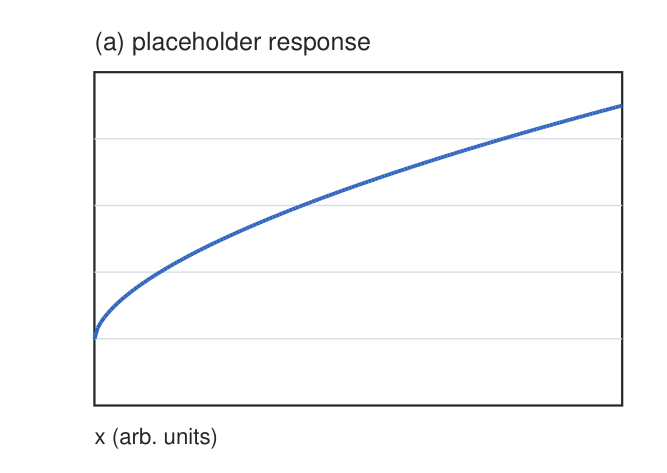
\includegraphics[width=\textwidth]{panel_a}
    \caption{First placeholder panel}\label{fig:panels:a}
  \end{subfigure}\hfill
  \begin{subfigure}[b]{0.48\textwidth}
    \centering
    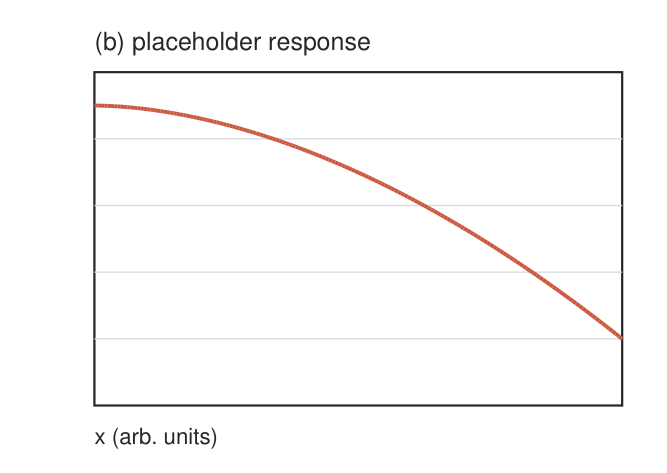
\includegraphics[width=\textwidth]{panel_b}
    \caption{Second placeholder panel}\label{fig:panels:b}
  \end{subfigure}
  \caption{A two-panel figure. (a,b) Placeholder panels drawn only to occupy
    space. The caption must sit on its own line, stay with its figure across a
    page break, and carry a live figure number.}
  \label{fig:panels}
\end{figure}

A single wide figure, and one supplied as a PDF so the converter has to
rasterise it---Word cannot embed PDF artwork.

\begin{figure}[htbp]
  \centering
  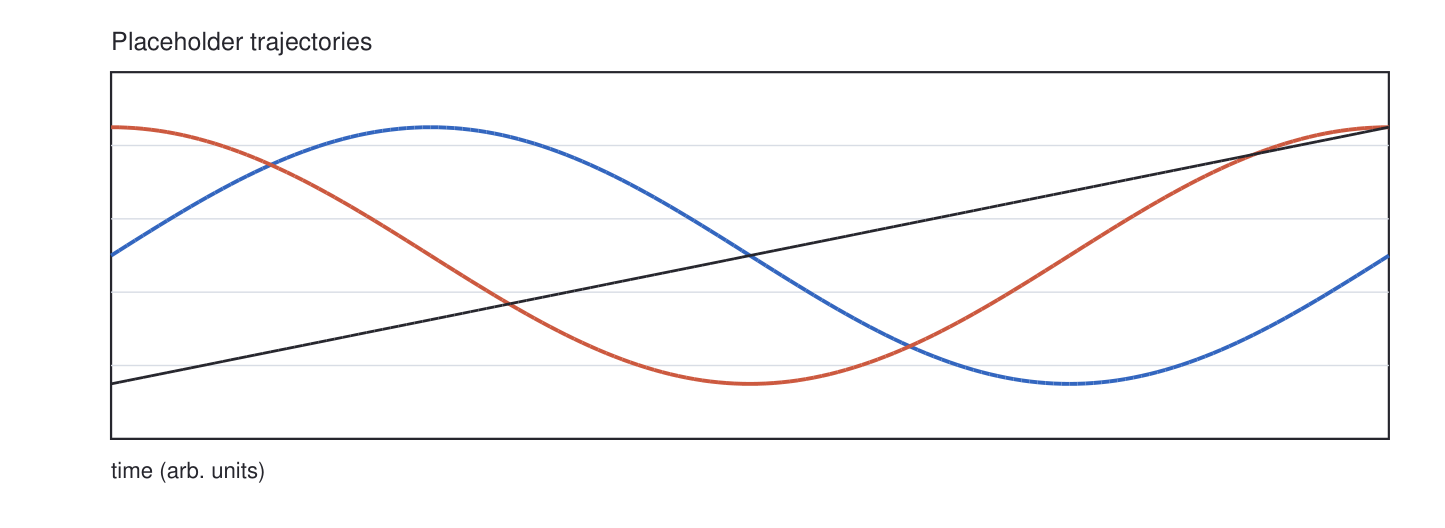
\includegraphics[width=\textwidth]{wide}
  \caption{A wide placeholder figure. Every image is scaled to one uniform width
    in the Word output, so the relative sizes of the source figures are not
    preserved.}
  \label{fig:wide}
\end{figure}

\begin{figure}[htbp]
  \centering
  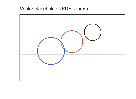
\includegraphics[width=0.6\textwidth]{vector.pdf}
  \caption{A figure supplied as PDF. The converter rasterises it at 300 dpi
    before handing the document to Word.}
  \label{fig:vector}
\end{figure}

\subsection{Tables}\label{sec:results:tables}

A booktabs table whose numeric columns hold pre-formatted values.

\begin{table}[htbp]
  \caption{Summary of placeholder measurements, reported as mean $\pm$ standard
    deviation across repeats.}
  \label{tab:summary}
  \begin{tabular}{@{}clcc@{}}
    \toprule
    Case & Label & Response & Count \\
    \midrule
    A & baseline          & $0.279 \pm 0.023$ & 50 \\
    B & uniform loading   & $0.281 \pm 0.024$ & 50 \\
    C & constant pressure & $0.372 \pm 0.044$ & 48 \\
    D & ramped input      & $0.316 \pm 0.030$ & 49 \\
    \botrule
  \end{tabular}
\end{table}

As reported in \cref{tab:summary}, case C differs from the baseline while the
others do not. The corresponding trajectories appear in \cref{fig:wide}, and the
derivation behind \cref{eq:energy} is given in \cref{app:derivation}.

\subsection{Discussion}

Text after the floats, to confirm that the body resumes cleanly. A URL in running
prose must become a clickable link with its trailing punctuation excluded: see
\url{https://doi.org/10.1000/placeholder.2020.101}. A bare URL inside
parentheses is the case that used to break
(\url{https://example.org/path_with_parens}).

\begin{appendices}

\section{Supporting derivation}\label{app:derivation}

Appendix headings are lettered rather than numbered, and cross-references to
them must say ``Appendix A''. Referring back to the body still works: see
\Cref{sec:theory} and \cref{eq:governing}.

Starting from \cref{eq:governing} and projecting onto the equilibrium profile,
\begin{equation}
  v_n \frac{\sigma}{\kappa} = \frac{1}{2} M E \int_0^1 h'(u)\,\hat{q}(u)\,du,
\end{equation}
which reduces, to leading order, to
\[
  v_n = M\left(W_2 - W_1\right).
\]
The unnumbered form above is deliberate: it is an intermediate step, not a
result, and it must not consume an equation number.

\section{Numerical parameters}\label{app:parameters}

A second appendix, so the converter has to recognise more than one appendix
title. The parameters used throughout are collected in \cref{tab:params}.

\begin{table}[htbp]
  \caption{Placeholder numerical parameters.}\label{tab:params}
  \begin{tabular}{@{}lll@{}}
    \toprule
    Symbol & Value & Units \\
    \midrule
    $M$      & 2.0                 & \si{\per\second} \\
    $\kappa$ & \num{1.0e-16}       & \si{\metre\squared\per\second} \\
    $E$      & 9.4                 & \si{\giga\pascal} \\
    \botrule
  \end{tabular}
\end{table}

The relative tolerance was \num{1e-6}, the grid spacing \qty{25}{\nano\metre},
and the domain \qtyproduct{10 x 1}{\micro\metre}. Robust statistics follow
\citet{noe2023}.

\end{appendices}

\bibliography{references}

\end{document}
